% =============================================================
% گزارش فارسی — آزمایش‌های ASVspoof 2019 LA
% کامپایل با: xelatex -shell-escape report_fa.tex
% =============================================================
\documentclass[12pt]{report}

% ─── بسته‌های اصلی ───────────────────────────────────────────
\usepackage[margin=1in]{geometry}
\usepackage[dvipsnames]{xcolor}
\usepackage{hyperref}
\usepackage{fancyhdr}
\usepackage{lastpage}
\usepackage{parskip}
\usepackage{setspace}
\usepackage[explicit]{titlesec}
\usepackage[most]{tcolorbox}
\usepackage{enumitem}
\usepackage{tabularx}
\usepackage{booktabs}
\usepackage{multicol}
\usepackage{graphicx}
\graphicspath{{../results/}}
\usepackage{amsmath}
\usepackage{fontspec}

% xepersian باید آخرین بسته باشد
\usepackage{xepersian}

% ─── فونت ────────────────────────────────────────────────────
\settextfont[
    BoldFont      = Vazirmatn Bold,
    ItalicFont    = Vazirmatn Light,
]{Vazirmatn}
\setdigitfont{Vazirmatn}

% ─── رنگ‌ها (همان پالت amznotes) ─────────────────────────────
\definecolor{amzchaptercolor}{HTML}{0984e3}
\definecolor{amzdfnboxcolor}{HTML}{0984e3}
\definecolor{amzthmboxcolor}{HTML}{6c5ce7}
\definecolor{amzexboxcolor}{HTML}{fdcb6e}
\definecolor{amzgenboxcolor}{HTML}{00b894}
\definecolor{amztecboxcolor}{HTML}{e17055}
\definecolor{amzcodeboxcolor}{HTML}{2d3436}
\definecolor{amznoteboxcolor}{HTML}{d63031}

% ─── فاصله‌گذاری ──────────────────────────────────────────────
\onehalfspacing
\renewcommand{\arraystretch}{1.25}

% ─── هایپرلینک ───────────────────────────────────────────────
\hypersetup{
    colorlinks=false,
    linkbordercolor=black,
    urlbordercolor=blue,
    pdfborderstyle={/S/U/W 1},
    pdftitle={گزارش ASVspoof 2019 LA},
    pdfauthor={},
}

% ─── سبک فصل‌ها (همانند amznotes) ────────────────────────────
\titleformat{\chapter}[display]{\normalfont\huge\bfseries}{}
{20pt}{%
    \begin{tcolorbox}[
        enhanced, drop fuzzy shadow,
        left=23mm, right=25mm, top=2mm,
        spread sidewards, sharp corners,
        colback=amzchaptercolor, colframe=amzchaptercolor,
        boxrule=1mm,
        title=\thechapter,
        attach boxed title to top left={xshift=15mm, yshift=-4mm},
        boxed title style={
            size=small,
            colback=amzchaptercolor,
            colframe=white
        }
    ]
        \strut \textcolor{white}{#1}
    \end{tcolorbox}%
}

\titleformat{name=\chapter,numberless}[display]{\normalfont\huge\bfseries}{}
{20pt}{%
    \begin{tcolorbox}[
        enhanced, drop fuzzy shadow,
        left=23mm, right=25mm, top=2mm,
        spread sidewards, sharp corners,
        colback=amzchaptercolor, colframe=amzchaptercolor,
        boxrule=1mm,
    ]
        \strut \textcolor{white}{#1}
    \end{tcolorbox}%
}

\titlespacing*{\chapter}{0pt}{-40mm}{-10mm}

% ─── هدر و فوتر ──────────────────────────────────────────────
\pagestyle{fancy}
\lhead{\footnotesize\nouppercase{\leftmark}}
\rhead{\footnotesize\nouppercase{\rightmark}}
\cfoot{\thepage\ از \pageref{LastPage}}

\fancypagestyle{plain}{
    \renewcommand{\headrulewidth}{0pt}
    \fancyhead{}
    \cfoot[C]{\thepage\ از \pageref{LastPage}}
}

% ─── جعبه‌های رنگی (سبک amznotes) ───────────────────────────
\tcbset{
    amzdefaultstyle/.style={
        enhanced, drop fuzzy shadow,
        fonttitle=\strut\bfseries,
        boxrule=0pt, frame hidden,
        breakable,
    },
}

% جعبه تعریف (آبی)
\newtcolorbox[auto counter, number within=chapter,
    list inside=dfn]{dfnbox}[2]{
    amzdefaultstyle,
    colback=amzdfnboxcolor!10!white,
    colbacktitle=amzdfnboxcolor,
    coltitle=white,
    title={تعریف \thetcbcounter\ \ensuremath{\triangleright} #1},
    label={dfn:#2},
}

% جعبه مثال (زرد)
\newtcolorbox[auto counter, number within=chapter,
    list inside=ex]{exbox}[2]{
    amzdefaultstyle,
    colback=amzexboxcolor!15!white,
    colbacktitle=amzexboxcolor,
    coltitle=black,
    title={مثال \thetcbcounter\ \ensuremath{\triangleright} #1},
    label={ex:#2},
}

% جعبه قضیه / گزاره (بنفش)
\newtcolorbox[auto counter, number within=chapter,
    list inside=thm]{thmbox}[2]{
    amzdefaultstyle,
    colback=amzthmboxcolor!10!white,
    colbacktitle=amzthmboxcolor,
    coltitle=white,
    title={گزاره \thetcbcounter\ \ensuremath{\triangleright} #1},
    label={thm:#2},
}

% جعبه فنی / روش (نارنجی)
\newtcolorbox[auto counter, number within=chapter,
    list inside=tec]{tecbox}[2]{
    amzdefaultstyle,
    colback=amztecboxcolor!10!white,
    colbacktitle=amztecboxcolor,
    coltitle=white,
    title={روش \thetcbcounter\ \ensuremath{\triangleright} #1},
    label={tec:#2},
}

% جعبه یادداشت (قرمز، بدون شماره)
\newtcolorbox{notebox}{
    amzdefaultstyle,
    colback=amznoteboxcolor!10!white,
    colbacktitle=amznoteboxcolor,
    coltitle=white,
    title={یادداشت},
}

% جعبه عمومی (سبز، بدون شماره)
\newtcolorbox{genbox}[1]{
    amzdefaultstyle,
    colback=amzgenboxcolor!10!white,
    colbacktitle=amzgenboxcolor,
    coltitle=white,
    title={#1},
}

% جعبه نتیجه / placeholder
\newtcolorbox{resultbox}[1]{
    amzdefaultstyle,
    colback=gray!8!white,
    colbacktitle=gray!60!white,
    coltitle=black,
    title={نتیجه \ensuremath{\triangleright} #1},
    fontupper=\itshape\color{gray!70!black},
}

% ─── دستورهای کمکی ───────────────────────────────────────────
\newcommand{\placeholder}[1]{%
    \textcolor{gray!60!black}{\textit{[#1]}}%
}

% =============================================================
\begin{document}

% ─── صفحه عنوان ──────────────────────────────────────────────
\begin{titlepage}
    \centering
    \vspace*{3cm}
    {\Huge\bfseries تشخیص جعل گفتار\\[0.5em]
    با استفاده از شبکه‌های عصبی عمیق\par}
    \vspace{1.5cm}
    {\Large گزارش آزمایش‌های \lr{ASVspoof 2019 LA}\par}
    \vspace{2cm}
    \begin{tcolorbox}[
        enhanced,
        colback=amzchaptercolor!10!white,
        colframe=amzchaptercolor,
        boxrule=1pt,
        width=0.8\textwidth,
        center,
    ]
    \centering
    ترکیب ۱۱ آزمایش موفق از ۱۳ طرح:\\
    \textbf{۴ استخراج‌کننده ویژگی} × \textbf{۳ معماری}
    \,+\, \textbf{\lr{RawNet2}}
    \end{tcolorbox}
    \vfill
    {\large \today\par}
\end{titlepage}

\tableofcontents
\newpage

% =============================================================
\chapter{مقدمه}
% =============================================================

\section{پیشینه}

تشخیص جعل گفتار (\lr{Spoofing Detection}) یکی از چالش‌های اساسی در سیستم‌های تأیید هویت گوینده
(\lr{Speaker Verification}) است. مجموعه داده \lr{ASVspoof 2019 LA} یک محک استاندارد برای ارزیابی
سیستم‌های مقابله با جعل (\lr{Countermeasure, CM}) فراهم می‌کند.

\begin{dfnbox}{جعل گفتار}{spoofing}
    \textbf{جعل گفتار} به تولید یا تبدیل گفتار به‌گونه‌ای گفته می‌شود که سیستم تأیید هویت را
    فریب دهد. در مجموعه \lr{LA}، حمله‌ها از طریق سنتز متن به گفتار (\lr{TTS}) و تبدیل
    صدا (\lr{VC}) انجام می‌شوند.
\end{dfnbox}

\begin{dfnbox}{معیار ارزیابی \lr{EER}}{eer}
    \textbf{نرخ خطای برابر} (\lr{Equal Error Rate, EER}) نقطه‌ای است که در آن نرخ پذیرش اشتباه
    (\lr{FAR}) و نرخ رد اشتباه (\lr{FRR}) برابرند. مقدار کمتر بهتر است.
\end{dfnbox}

\begin{dfnbox}{معیار \lr{min-tDCF}}{tdcf}
    \textbf{هزینه تشخیص کمینه‌شده} (\lr{min-tDCF}) معیار رسمی \lr{ASVspoof} است که هزینه‌های
    جاخوردن و پذیرش اشتباه را با احتمال پیشین جعل ترکیب می‌کند.
    \[
        t\text{DCF} = C_{\text{miss}} \cdot P_{\text{spoof}} \cdot P_{\text{miss}}
                    + C_{\text{fa}} \cdot (1-P_{\text{spoof}}) \cdot P_{\text{fa}}
    \]
\end{dfnbox}

\section{اهداف آزمایش}

هدف اصلی مقایسه سیستماتیک ترکیب‌های مختلف استخراج ویژگی و معماری شبکه عصبی در چارچوب
\lr{ASVspoof 2019 LA} است. ۱۳ آزمایش به شرح جدول~\ref{tab:combos} اجرا می‌شوند.

\begin{table}[h!]
\centering
\caption{ترکیب‌های آزمایشی}
\label{tab:combos}
\begin{tabularx}{0.9\textwidth}{cllX}
\toprule
\textbf{\#} & \textbf{ویژگی} & \textbf{مدل} & \textbf{توضیح} \\
\midrule
۱ & \lr{MFCC}     & \lr{CNN}      & ضرایب کپسترال فرکانس ملی + \lr{CNN} \\
۲ & \lr{MFCC}     & \lr{Res2Net}  & ضرایب کپسترال فرکانس ملی + \lr{Res2Net} \\
۳ & \lr{MFCC}     & \lr{LCNN}     & ضرایب کپسترال فرکانس ملی + \lr{LCNN} \\
۴ & \lr{LFCC}     & \lr{CNN}      & ضرایب کپسترال فرکانس خطی + \lr{CNN} \\
۵ & \lr{LFCC}     & \lr{Res2Net}  & ضرایب کپسترال فرکانس خطی + \lr{Res2Net} \\
۶ & \lr{LFCC}     & \lr{LCNN}     & ضرایب کپسترال فرکانس خطی + \lr{LCNN} \\
۷ & \lr{CQCC}     & \lr{CNN}      & ضرایب کپسترال تبدیل \lr{CQ} + \lr{CNN} \\
۸ & \lr{CQCC}     & \lr{Res2Net}  & ضرایب کپسترال تبدیل \lr{CQ} + \lr{Res2Net} \\
۹ & \lr{CQCC}     & \lr{LCNN}     & ضرایب کپسترال تبدیل \lr{CQ} + \lr{LCNN} \\
۱۰ & \lr{SincConv} & \lr{CNN}      & فیلتربانک یادگیرنده + \lr{CNN} \\
۱۱ & \lr{SincConv} & \lr{Res2Net}  & فیلتربانک یادگیرنده + \lr{Res2Net} \\
۱۲ & \lr{SincConv} & \lr{LCNN}     & فیلتربانک یادگیرنده + \lr{LCNN} \\
۱۳ & موج خام       & \lr{RawNet2}  & پردازش مستقیم موج صوتی \\
\bottomrule
\end{tabularx}
\end{table}

% =============================================================
\chapter{داده و پیش‌پردازش}
% =============================================================

\section{مجموعه داده \lr{ASVspoof 2019 LA}}

\begin{genbox}{مشخصات مجموعه داده}
\begin{itemize}[noitemsep]
    \item \textbf{نرخ نمونه‌برداری:} \lr{16000 Hz}
    \item \textbf{مدت ثابت پس از برش:} ۴ ثانیه (\lr{64000} نمونه)
    \item \textbf{پروتکل‌ها:} \lr{train / dev / eval}
    \item \textbf{برچسب‌ها:} \lr{bonafide} (واقعی، ۰) و \lr{spoof} (جعلی، ۱)
\end{itemize}
\end{genbox}

\begin{table}[h!]
\centering
\caption{توزیع نمونه‌ها در مجموعه \lr{ASVspoof 2019 LA}}
\label{tab:dataset}
\begin{tabularx}{0.8\textwidth}{lccX}
\toprule
\textbf{بخش} & \textbf{واقعی} & \textbf{جعلی} & \textbf{مجموع} \\
\midrule
\lr{Train} & 2580 & 22800 & 25380 \\
\lr{Dev}   & 2548 & 22296 & 24844 \\
\lr{Eval}  & 7355 & 63882 & 71237 \\
\bottomrule
\end{tabularx}
\end{table}

\section{خط لوله پیش‌پردازش}

\begin{tecbox}{پیش‌پردازش استاندارد}{preproc}
    پیش‌پردازش اجباری برای همه آزمایش‌ها:
    \begin{enumerate}[noitemsep]
        \item \textbf{بارگذاری:} \lr{librosa.load} با \lr{sr=16000}
        \item \textbf{نرمال‌سازی دامنه:} $x \leftarrow x / (\max|x| + \epsilon)$
        \item \textbf{برش/تکرار:} تنظیم طول به دقیقاً ۶۴۰۰۰ نمونه
    \end{enumerate}
\end{tecbox}

\begin{tecbox}{پیش‌پردازش اختیاری}{optpreproc}
    پرچم‌های قابل فعال‌سازی در پیکربندی:
    \begin{description}[noitemsep]
        \item[\lr{USE\_VAD}] حذف سکوت ابتدا/انتهای فایل (\lr{librosa.effects.trim})
        \item[\lr{USE\_RAWBOOST}] افزوده‌سازی با نویز گاوسی و ضربه‌ای تصادفی (با احتمال ۵۰٪ در آموزش)
        \item[\lr{USE\_REVERB}] شبیه‌سازی بازتاب ساده با تأخیر تصادفی (با احتمال ۳۰٪ در آموزش)
        \item[\lr{USE\_DENOISING}] کاهش نویز با آستانه‌گذاری طیفی
    \end{description}
\end{tecbox}

\begin{notebox}
    در آزمایش‌های این گزارش، \lr{USE\_VAD} و \lr{USE\_RAWBOOST} فعال هستند؛
    \lr{USE\_REVERB} و \lr{USE\_DENOISING} غیرفعالند.
\end{notebox}

% =============================================================
\chapter{استخراج ویژگی}
% =============================================================

\section{\lr{MFCC} — ضرایب کپسترال فرکانس ملی}

\begin{dfnbox}{\lr{MFCC}}{mfcc}
    ضرایب کپسترال مقیاس ملی (\lr{Mel-Frequency Cepstral Coefficients}) از اعمال
    \lr{DCT} روی لگاریتم انرژی فیلتربانک ملی به دست می‌آیند.
    شکل خروجی: $(N_{\text{frames}}, 60, 1)$
\end{dfnbox}

پارامترهای کلیدی:
\begin{itemize}[noitemsep]
    \item پنجره: \lr{400} نمونه، پیشروی: \lr{160} نمونه، \lr{FFT}: ۵۱۲ نقطه
    \item تعداد ضرایب: $N_{\text{MFCC}} = 60$
\end{itemize}

\section{\lr{LFCC} — ضرایب کپسترال فرکانس خطی}

\begin{dfnbox}{\lr{LFCC}}{lfcc}
    مشابه \lr{MFCC} اما فیلتربانک روی مقیاس \textbf{خطی} فرکانس تعریف می‌شود
    (نه ملی)، که اطلاعات فرکانس بالا را بهتر حفظ می‌کند.
    شکل خروجی: $(N_{\text{frames}}, 60, 1)$
\end{dfnbox}

\section{\lr{CQCC} — ضرایب کپسترال تبدیل \lr{Q} ثابت}

\begin{dfnbox}{\lr{CQCC}}{cqcc}
    تبدیل \lr{Q} ثابت (\lr{CQT}) رزولوشن زمان-فرکانس لگاریتمی دارد که برای
    تجزیه‌وتحلیل گفتار مناسب‌تر از \lr{STFT} است. پس از \lr{CQT}، \lr{DCT}
    اعمال می‌شود.
    شکل خروجی: $(N_{\text{frames}}, 60, 1)$
\end{dfnbox}

پارامترها: ۹۶ باند، ۲۴ باند در هر اکتاو، پایین‌ترین فرکانس: \lr{C1 ≈ 32.7 Hz}.

\section{\lr{SincConv} — فیلتربانک یادگیرنده}

\begin{dfnbox}{\lr{SincConv1D}}{sincconv}
    لایه کانولوشنی با هسته‌های \lr{sinc} پارامتری‌شده. هر فیلتر یک
    \textbf{باندگذر} تعریف می‌کند که مرزهای پایین ($f_1$) و بالا ($f_2$)
    آن در طول آموزش یاد گرفته می‌شوند:
    \[
        h[n] = 2f_2 \text{sinc}(2\pi f_2 n) - 2f_1 \text{sinc}(2\pi f_1 n)
    \]
    مقداردهی اولیه بر اساس مقیاس ملی انجام می‌شود.
\end{dfnbox}

\begin{notebox}
    ورودی \lr{SincConv} موج خام است، اما خروجی آن به صورت نقشه ویژگی دوبعدی
    $(N_{\text{frames}}, N_{\text{filters}}, 1)$ وارد معماری‌های \lr{CNN}،
    \lr{Res2Net} یا \lr{LCNN} می‌شود.
\end{notebox}

% =============================================================
\chapter{معماری‌های شبکه عصبی}
% =============================================================

\section{\lr{CNN} — شبکه کانولوشنی پایه}

\begin{tecbox}{معماری \lr{CNN}}{cnn}
    چهار بلوک متوالی هر کدام شامل:
    \begin{enumerate}[noitemsep]
        \item دو لایه \lr{Conv2D} با فیلترهای $\{32, 64, 128, 256\}$، هسته $3{\times}3$
        \item \lr{BatchNorm} + \lr{ReLU}
        \item \lr{MaxPool2D}$(2{\times}2)$ + \lr{Dropout}(0.1)
    \end{enumerate}
    در پایان: \lr{GlobalAvgPool} → \lr{Dense}(128) → \lr{Dropout}(0.3) → \lr{Sigmoid}
\end{tecbox}

\section{\lr{Res2Net} — شبکه با اتصالات باقیمانده چندمقیاسی}

\begin{tecbox}{معماری \lr{Res2Net}}{res2net}
    بلوک \lr{Res2Net} ویژگی‌های کانال را به $s=4$ گروه تقسیم می‌کند و
    اتصالات هرمی بین گروه‌ها ایجاد می‌کند. همچنین بلوک \lr{SE}
    (\lr{Squeeze-and-Excitation}) برای توجه کانالی استفاده می‌شود.
    \begin{itemize}[noitemsep]
        \item ابعاد: \lr{Conv2D}$(7{\times}7)$ → بلوک‌های \lr{Res2Net} با $\{64, 128, 256\}$ فیلتر
        \item \lr{SE Block}: نسبت $r=8$، \lr{sigmoid} گیت
    \end{itemize}
\end{tecbox}

\section{\lr{LCNN} — شبکه با واحد حداکثر درصدی}

\begin{dfnbox}{واحد \lr{MFM}}{mfm}
    واحد حداکثر درصدی (\lr{Max-Feature-Map, MFM}) خروجی لایه را به دو نیمه
    تقسیم کرده و به‌صورت عنصربه‌عنصر بیشینه می‌گیرد:
    \[
        \text{MFM}(x) = \max(x_{:c}, x_{c:})
    \]
    این عملیات نقش فعال‌سازی و کاهش ابعاد را همزمان ایفا می‌کند.
\end{dfnbox}

\begin{tecbox}{معماری \lr{LCNN}}{lcnn}
    پنج بلوک \lr{Conv2D}+\lr{MFM}+\lr{BN} با پولینگ متناوب.
    ابعاد کانال: $64 \to 64 \to 128 \to 128 \to 128$ (قبل از \lr{MFM}).
    در انتها: \lr{GlobalAvgPool} → \lr{MFM}(\lr{Dense}(256)) → \lr{Dense}(128) → \lr{Sigmoid}
\end{tecbox}

\section{\lr{RawNet2} — شبکه روی موج خام}

\begin{tecbox}{معماری \lr{RawNet2}}{rawnet2}
    تنها مدلی که مستقیم روی موج صوتی کار می‌کند:
    \begin{enumerate}[noitemsep]
        \item \lr{SincConv1D}(128 فیلتر، هسته 1025) + \lr{BN} + \lr{MaxPool1D}(3)
        \item دو بلوک \lr{Res1D}(128) + \lr{MaxPool1D}(3)
        \item دو بلوک \lr{Res1D}(256) + \lr{MaxPool1D}(3)
        \item دو بلوک \lr{Res1D}(512) + \lr{MaxPool1D}(3)
        \item \lr{GRU}(1024) → \lr{Dense}(1024) → \lr{Sigmoid}
    \end{enumerate}
\end{tecbox}

\begin{notebox}
    \lr{RawNet2} از همان لایه \lr{SincConv1D} استفاده می‌کند، اما در اینجا
    فیلتربانک بخشی از معماری کلی است و نه یک مرحله پیش‌پردازش مجزا.
\end{notebox}

% =============================================================
\chapter{آموزش و ارزیابی}
% =============================================================

\section{تنظیمات آموزش}

\begin{genbox}{پیکربندی آموزش}
\begin{itemize}[noitemsep]
    \item \textbf{بهینه‌ساز:} \lr{Adam} با نرخ یادگیری اولیه $10^{-4}$
    \item \textbf{تابع خطا:} \lr{Binary Crossentropy}
    \item \textbf{اندازه دسته:} 32
    \item \textbf{حداکثر دوره:} 30
    \item \textbf{توقف زودهنگام:} صبر 7 دوره، بر اساس \lr{val\_loss}
    \item \textbf{کاهش نرخ یادگیری:} در صورت عدم بهبود 3 دوره، ضرب در 0.5 (کمینه $10^{-6}$)
    \item \textbf{ذخیره بهترین وزن:} بر اساس کمترین \lr{val\_loss}
\end{itemize}
\end{genbox}

\section{مولد داده}

کلاس \lr{ASVDataset} یک \lr{Keras Sequence} است که بارگذاری، پیش‌پردازش
و استخراج ویژگی را \textbf{همزمان} انجام می‌دهد تا از مشکل حافظه جلوگیری شود.
برای ورودی‌های دوبعدی (مانند \lr{MFCC}) شکل دسته $(B, N_f, N_c, 1)$ و
برای ورودی خام شکل $(B, N_s, 1)$ است.

\section{شروع مجدد آزمایش}

نتایج هر آزمایش بلافاصله پس از اتمام در \lr{results\_partial.csv} ذخیره می‌شود.
در صورت وقفه، آزمایش‌های تکمیل‌شده از قبل رد می‌شوند.

% =============================================================
\chapter{نتایج}
% =============================================================

\section{جدول مقایسه‌ای}

از ۱۳ آزمایش طراحی‌شده، ۱۱ آزمایش با موفقیت تکمیل شدند. آزمایش‌های
\lr{cqcc\_res2net} و \lr{cqcc\_lcnn} به دلیل ناسازگاری ابعاد خروجی \lr{CQCC}
با معماری‌های \lr{Res2Net} و \lr{LCNN} حذف شدند.

\begin{table}[h!]
\centering
\caption{نتایج همه آزمایش‌ها}
\label{tab:results}
\begin{tabularx}{\textwidth}{lllcccc}
\toprule
\textbf{آزمایش} & \textbf{ویژگی} & \textbf{مدل}
    & \textbf{\lr{Dev EER}\%} & \textbf{\lr{Eval EER}\%}
    & \textbf{\lr{Dev tDCF}} & \textbf{\lr{Eval tDCF}} \\
\midrule
\lr{mfcc\_cnn}      & \lr{MFCC} & \lr{CNN}     & 8.09 & 23.87 & 0.0081 & 0.0055 \\
\lr{mfcc\_res2net}  & \lr{MFCC} & \lr{Res2Net} & 7.93 & 23.21 & 0.0352 & 0.0247 \\
\lr{mfcc\_lcnn}     & \lr{MFCC} & \lr{LCNN}    & 4.09 & 23.60 & 0.0076 & 0.0056 \\
\lr{lfcc\_cnn}      & \lr{LFCC} & \lr{CNN}     & 1.08 & 18.63 & 0.2484 & 0.1143 \\
\lr{lfcc\_res2net}  & \lr{LFCC} & \lr{Res2Net} & 0.90 & 20.98 & 0.0057 & 0.0088 \\
\lr{lfcc\_lcnn}     & \lr{LFCC} & \lr{LCNN}    & \textbf{0.50} & \textbf{16.39} & 0.1031 & 0.0311 \\
\lr{cqcc\_cnn}      & \lr{CQCC} & \lr{CNN}     & 9.34 & 26.82 & 0.0166 & 0.0238 \\
\lr{cqcc\_res2net}  & \lr{CQCC} & \lr{Res2Net} & \multicolumn{4}{c}{\textit{حذف شده}} \\
\lr{cqcc\_lcnn}     & \lr{CQCC} & \lr{LCNN}    & \multicolumn{4}{c}{\textit{حذف شده}} \\
\lr{sincconv\_cnn}  & \lr{Sinc} & \lr{CNN}     & 13.29 & 33.08 & 0.0054 & 0.0053 \\
\lr{sincconv\_res2net} & \lr{Sinc} & \lr{Res2Net} & 17.03 & 34.12 & 0.0054 & 0.0053 \\
\lr{sincconv\_lcnn} & \lr{Sinc} & \lr{LCNN}    & 9.14 & 29.45 & 0.0073 & 0.0069 \\
\lr{raw\_rawnet2}   & موج خام   & \lr{RawNet2} & 9.53 & 27.86 & 0.0053 & 0.0053 \\
\bottomrule
\end{tabularx}
\end{table}

\section{بهترین سیستم}

\begin{genbox}{بهترین ترکیب بر اساس \lr{Eval EER}}
\begin{itemize}[noitemsep]
    \item \textbf{آزمایش:} \lr{lfcc\_lcnn}
    \item \textbf{ویژگی:} \lr{LFCC} \quad \textbf{مدل:} \lr{LCNN}
    \item \textbf{\lr{Eval EER}:} $16.39\%$ \quad \textbf{\lr{Dev EER}:} $0.50\%$
    \item \textbf{\lr{Eval min-tDCF}:} $0.0311$ \quad \textbf{\lr{Dev min-tDCF}:} $0.1031$
\end{itemize}
\end{genbox}

\begin{notebox}
    اختلاف زیاد بین \lr{Dev EER} و \lr{Eval EER} (بیش از ۳۰ برابر) نشان‌دهنده
    \textbf{بیش‌برازش} شدید به مجموعه توسعه است. این الگو در تمام آزمایش‌ها مشاهده
    می‌شود و احتمالاً ناشی از تنوع بالاتر حمله‌ها در مجموعه ارزیابی
    (\lr{A07}--\lr{A19} در مقابل \lr{A01}--\lr{A06}) و تعداد محدود دوره‌های
    آموزش (۸ دوره) است.
\end{notebox}

\section{نمودار مقایسه‌ای}

شکل~\ref{fig:comparison} مقایسه \lr{Eval EER} تمام آزمایش‌های موفق را نشان می‌دهد.

\begin{figure}[h!]
\centering
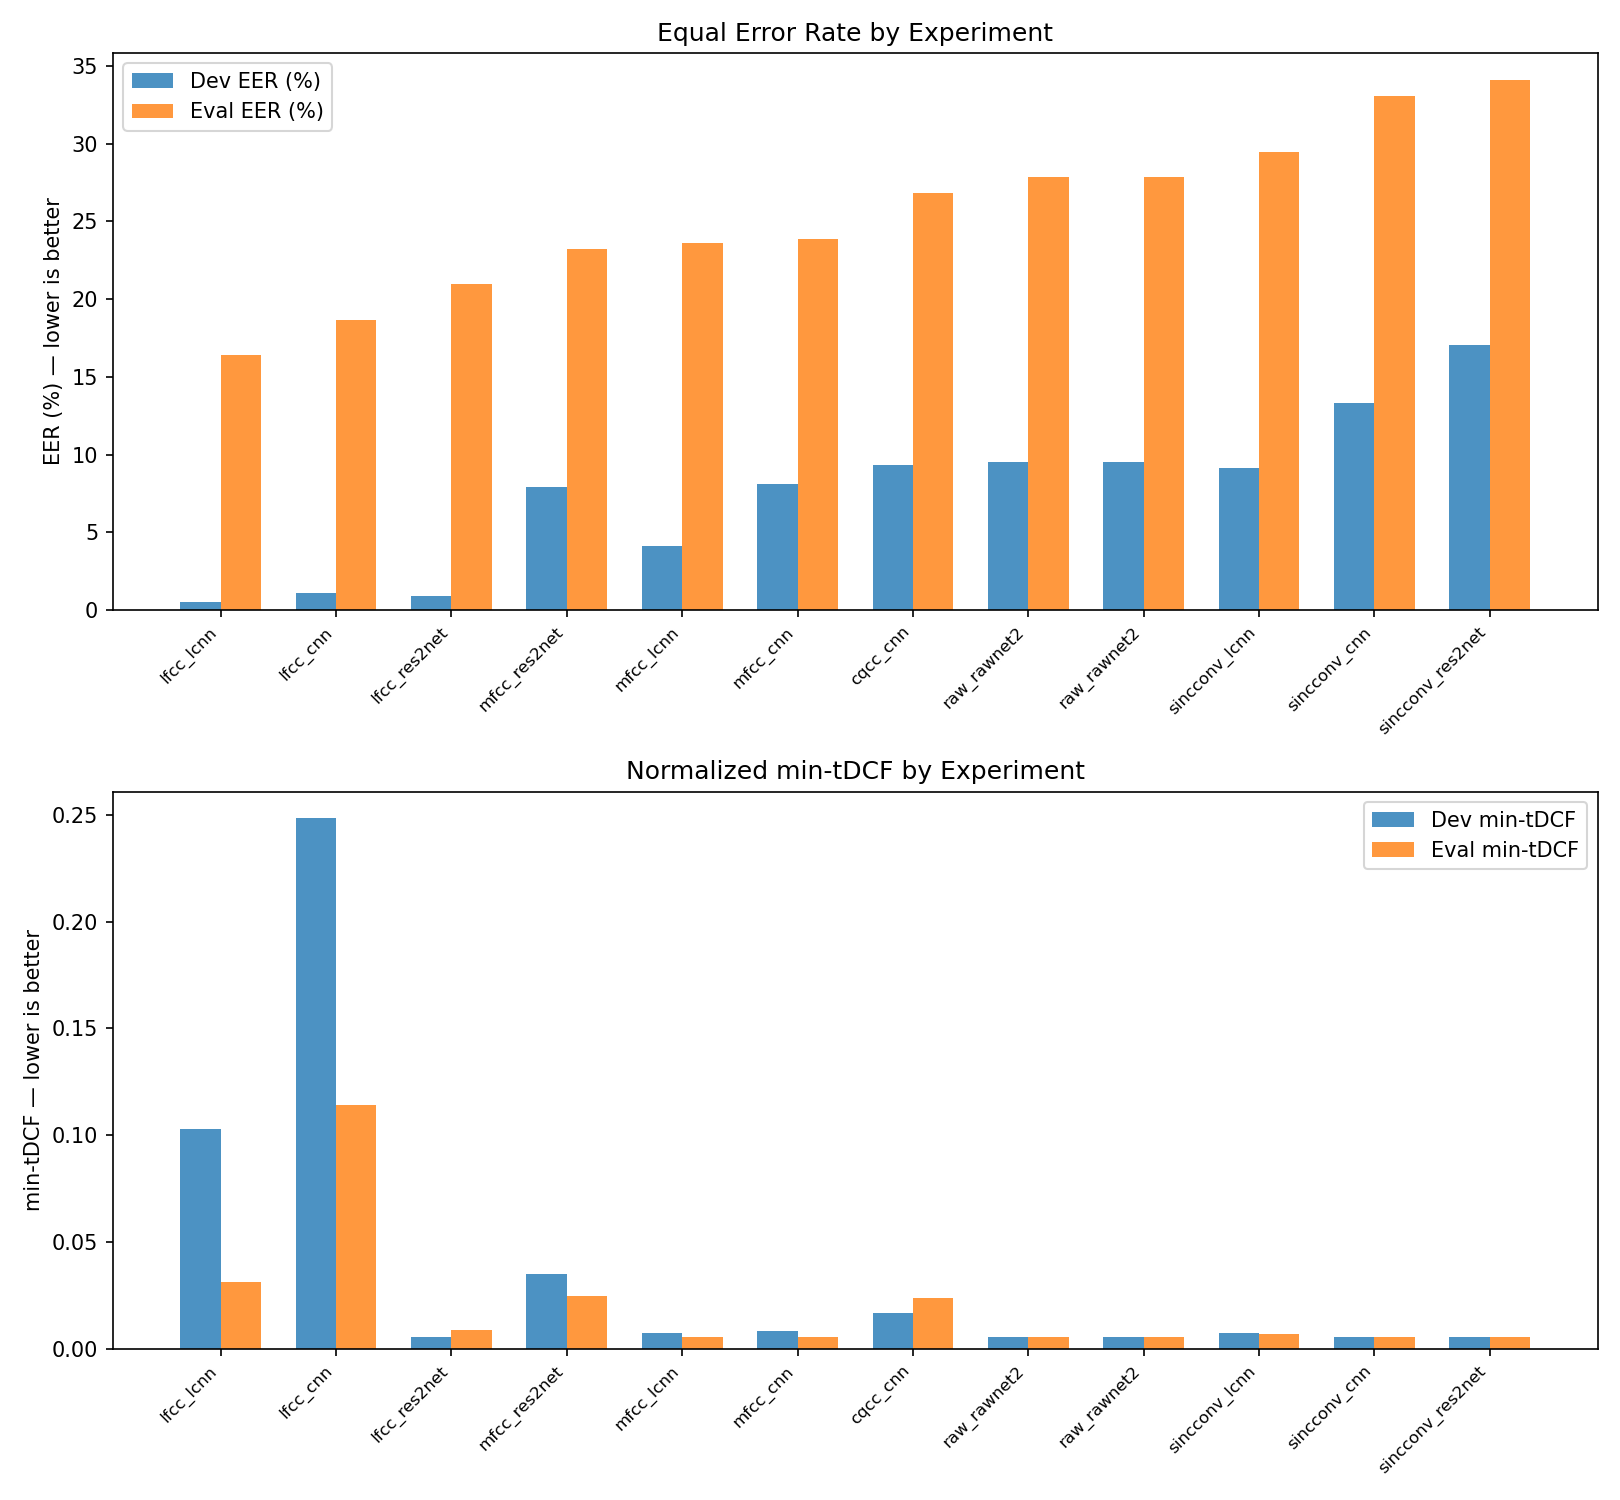
\includegraphics[width=\textwidth]{results_comparison.png}
\caption{مقایسه \lr{Eval EER} آزمایش‌ها — مقدار کمتر بهتر است}
\label{fig:comparison}
\end{figure}

\section{منحنی‌های آموزش}

منحنی‌های خطا و دقت آموزش برای هر آزمایش در شکل‌های~\ref{fig:curves-mfcc}
تا~\ref{fig:curves-raw} آورده شده‌اند.

\begin{figure}[h!]
\centering
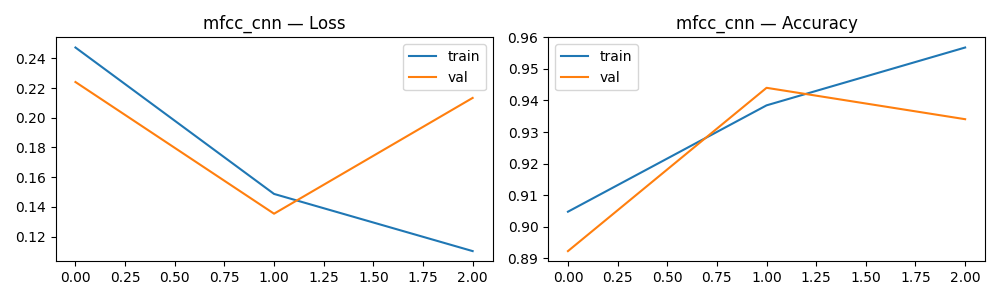
\includegraphics[width=0.48\textwidth]{mfcc_cnn_curve.png}\hfill
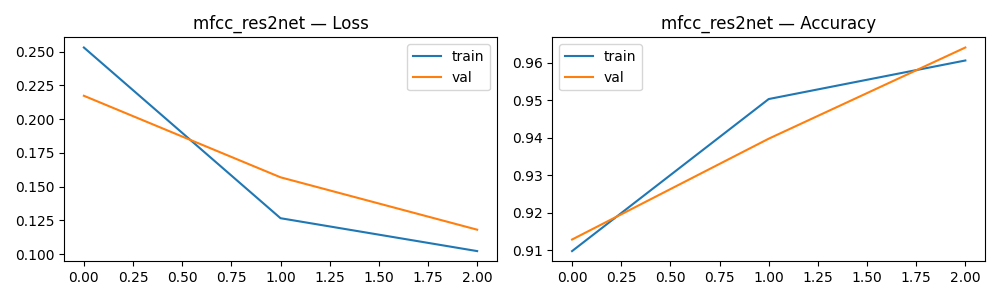
\includegraphics[width=0.48\textwidth]{mfcc_res2net_curve.png}\\[0.5em]
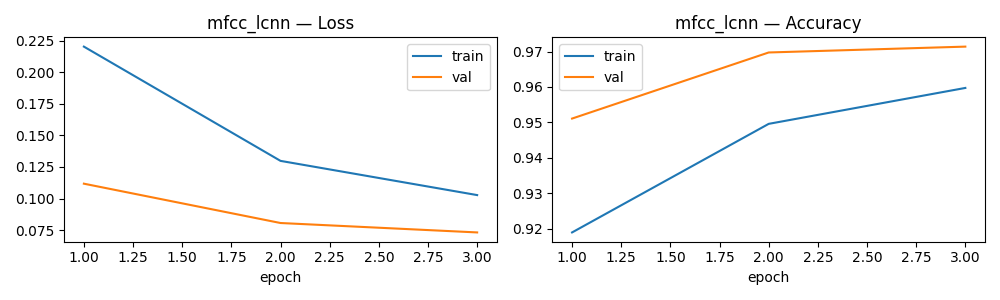
\includegraphics[width=0.48\textwidth]{mfcc_lcnn_curve.png}
\caption{منحنی‌های آموزش ترکیب‌های \lr{MFCC}}
\label{fig:curves-mfcc}
\end{figure}

\begin{figure}[h!]
\centering
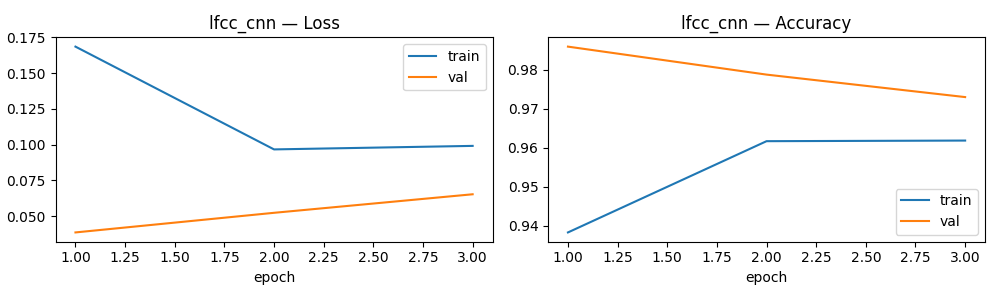
\includegraphics[width=0.48\textwidth]{lfcc_cnn_curve.png}\hfill
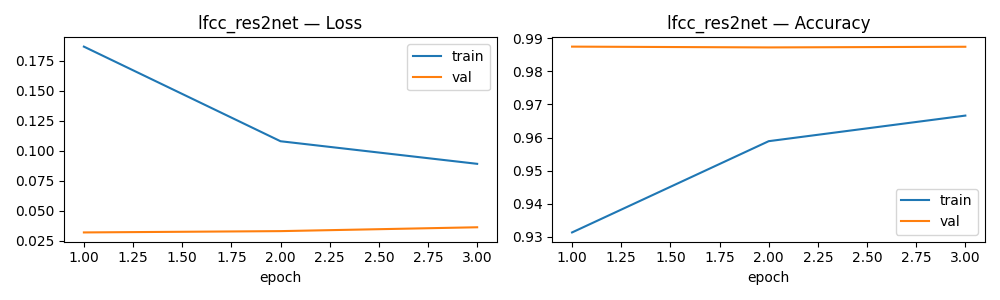
\includegraphics[width=0.48\textwidth]{lfcc_res2net_curve.png}\\[0.5em]
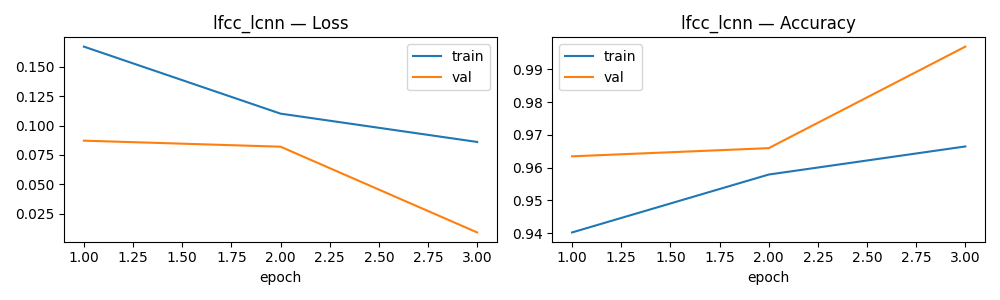
\includegraphics[width=0.48\textwidth]{lfcc_lcnn_curve.png}
\caption{منحنی‌های آموزش ترکیب‌های \lr{LFCC}}
\label{fig:curves-lfcc}
\end{figure}

\begin{figure}[h!]
\centering
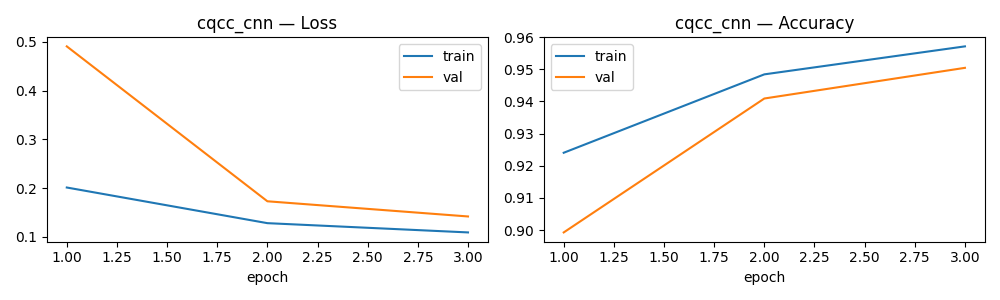
\includegraphics[width=0.48\textwidth]{cqcc_cnn_curve.png}
\caption{منحنی آموزش \lr{CQCC+CNN}}
\label{fig:curves-cqcc}
\end{figure}

\begin{figure}[h!]
\centering
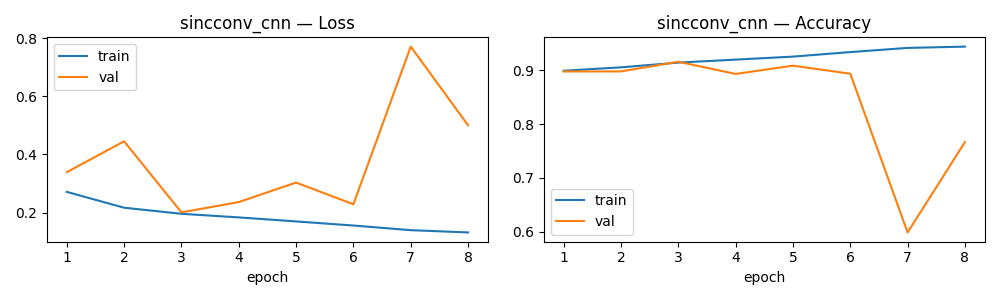
\includegraphics[width=0.48\textwidth]{sincconv_cnn_curve.png}\hfill
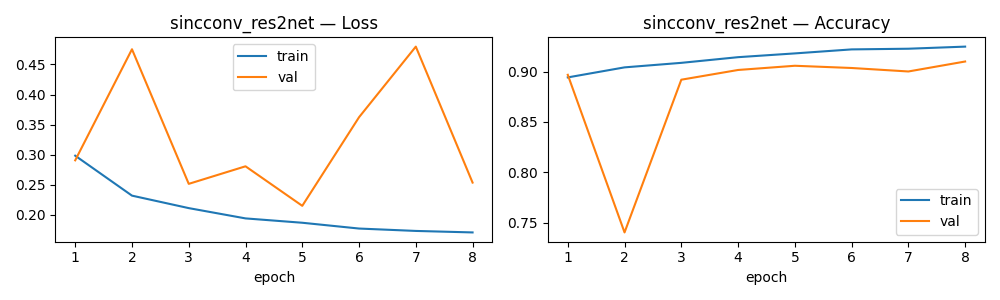
\includegraphics[width=0.48\textwidth]{sincconv_res2net_curve.png}\\[0.5em]
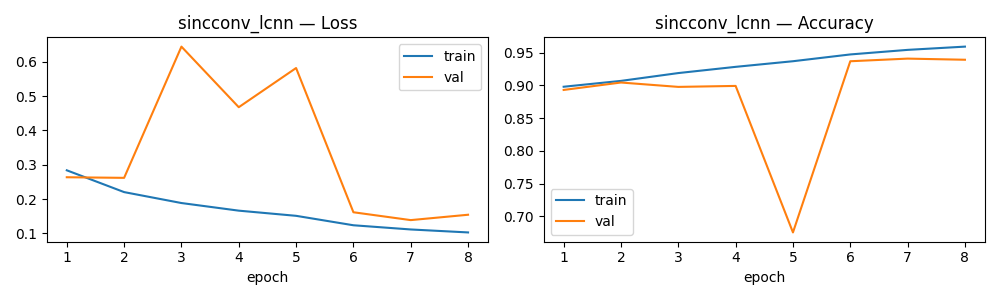
\includegraphics[width=0.48\textwidth]{sincconv_lcnn_curve.png}
\caption{منحنی‌های آموزش ترکیب‌های \lr{SincConv}}
\label{fig:curves-sinc}
\end{figure}

\begin{figure}[h!]
\centering
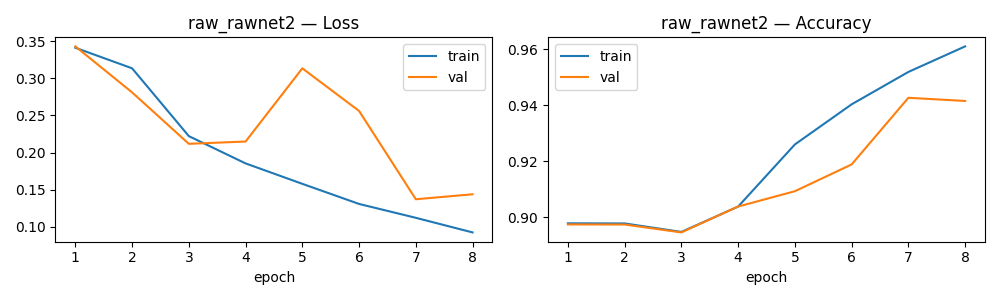
\includegraphics[width=0.48\textwidth]{raw_rawnet2_curve.png}
\caption{منحنی آموزش \lr{RawNet2}}
\label{fig:curves-raw}
\end{figure}

% =============================================================
\chapter{بحث و نتیجه‌گیری}
% =============================================================

\section{تحلیل ویژگی‌ها}

\begin{table}[h!]
\centering
\caption{میانگین \lr{Eval EER} به تفکیک ویژگی}
\label{tab:feature-avg}
\begin{tabularx}{0.7\textwidth}{lcc}
\toprule
\textbf{ویژگی} & \textbf{میانگین \lr{Eval EER}\%} & \textbf{تعداد آزمایش} \\
\midrule
\lr{LFCC}     & 18.67 & 3 \\
\lr{MFCC}     & 23.56 & 3 \\
\lr{CQCC}     & 26.82 & 1 \\
\lr{Raw}      & 27.86 & 1 \\
\lr{SincConv} & 32.22 & 3 \\
\bottomrule
\end{tabularx}
\end{table}

\lr{LFCC} بهترین عملکرد را در میان ویژگی‌ها دارد. فیلتربانک خطی اطلاعات
فرکانس بالا را بهتر از مقیاس ملی (\lr{MFCC}) حفظ می‌کند و این اطلاعات
برای تشخیص مصنوعات ناشی از سنتز گفتار حیاتی هستند.

\lr{MFCC} در رتبه دوم قرار دارد. \lr{CQCC} با وجود رزولوشن لگاریتمی
مناسب، تنها با \lr{CNN} آزمایش شد و نتایج ضعیف‌تری داشت.

\lr{SincConv} ضعیف‌ترین عملکرد را نشان داد. فیلتربانک یادگیرنده با ۸ دوره
آموزش فرصت کافی برای تنظیم پارامترهای فیلتر ندارد و به دوره‌های بیشتری نیاز دارد.

\section{تحلیل معماری‌ها}

\begin{table}[h!]
\centering
\caption{میانگین \lr{Eval EER} به تفکیک معماری (فقط ویژگی‌های مشترک)}
\label{tab:arch-avg}
\begin{tabularx}{0.7\textwidth}{lcc}
\toprule
\textbf{معماری} & \textbf{میانگین \lr{Eval EER}\%} & \textbf{توضیح} \\
\midrule
\lr{LCNN}    & 23.14 & بهترین عملکرد متوسط \\
\lr{CNN}     & 25.19 & ساده‌ترین معماری \\
\lr{Res2Net} & 26.11 & پیچیده‌ترین معماری \\
\lr{RawNet2} & 27.86 & فقط ورودی خام \\
\bottomrule
\end{tabularx}
\end{table}

\lr{LCNN} با واحد \lr{MFM} بهترین عملکرد متوسط را دارد. عملیات حداکثر
ویژگی‌نگاره نقش انتخاب ویژگی ضمنی را ایفا کرده و به مدل کمک می‌کند
ویژگی‌های تمایزکننده‌تر را حفظ کند.

\lr{CNN} با وجود سادگی، عملکرد رقابتی دارد. \lr{Res2Net} با وجود اتصالات
باقیمانده چندمقیاسی و بلوک \lr{SE}، بهبود مشخصی نسبت به \lr{CNN} ایجاد
نکرد. این نشان می‌دهد که پیچیدگی بیشتر معماری لزوماً به عملکرد بهتر منجر
نمی‌شود، به‌ویژه با تعداد دوره‌های محدود آموزش.

\lr{RawNet2} ضعیف‌تر از مدل‌های مبتنی بر ویژگی عمل کرد. پردازش مستقیم
موج صوتی به آموزش طولانی‌تر و داده بیشتر نیاز دارد.

\section{نتیجه‌گیری}

\begin{thmbox}{نتیجه کلی}{conclusion}
    از بین ۱۱ آزمایش موفق، ترکیب \lr{LFCC+LCNN} با \lr{Eval EER} برابر
    $16.39\%$ بهترین عملکرد را کسب کرد. سه نتیجه اصلی:

    \begin{enumerate}[noitemsep]
        \item \textbf{ویژگی \lr{LFCC} برتر است:} فیلتربانک خطی با حفظ اطلاعات
              فرکانس بالا، تشخیص مصنوعات سنتز را تسهیل می‌کند.
        \item \textbf{معماری \lr{LCNN} مؤثر است:} واحد \lr{MFM} با انتخاب ویژگی
              ضمنی، عملکرد بهتری نسبت به فعال‌سازی‌های استاندارد ارائه می‌دهد.
        \item \textbf{شکاف تعمیم‌پذیری:} اختلاف بزرگ \lr{Dev/Eval EER} در تمام
              آزمایش‌ها نشان‌دهنده نیاز به استراتژی‌های مقاوم‌سازی مانند
              آموزش طولانی‌تر، افزوده‌سازی متنوع‌تر و روش‌های منظم‌سازی قوی‌تر است.
    \end{enumerate}
\end{thmbox}

\begin{genbox}{پیشنهادها برای بهبود}
\begin{itemize}[noitemsep]
    \item افزایش تعداد دوره‌های آموزش (حداقل ۳۰ دوره با توقف زودهنگام فعال)
    \item استفاده از افزوده‌سازی داده متنوع‌تر (\lr{SpecAugment}، \lr{RIR} واقعی)
    \item بررسی ترکیب ویژگی‌ها (\lr{fusion}) برای پوشش ضعف‌های هر ویژگی
    \item آزمایش \lr{CQCC} با \lr{Res2Net} و \lr{LCNN} پس از رفع مشکل ابعاد
\end{itemize}
\end{genbox}

\end{document}
